\documentclass[a4paper, 12pt]{article}

\usepackage[english]{babel}
\usepackage[utf8]{inputenc}
\usepackage{graphicx}
\usepackage{makeidx}
\usepackage{float}
\usepackage{hyperref}
\usepackage[parfill]{parskip}

\title{Relazione Tecnologie Web 2014}
\author{Andrea Giacomo Baldan, Alberto De Agostini}
\date{3 Luglio 2014}
% sistemare img
\makeindex %fa l'indice automatico
\begin{document}
\maketitle

\begin{itemize}
\item E-mail referenti
  \begin{itemize}
  \item \emph{E-mail: a.g.baldan@gmail.com}
  \item \emph{E-mail: albertodeagostini88@gmail.com}
  \end{itemize}
\item Specifiche
  \begin{itemize}
  \item \emph{URL sito: http://tecnologie-web.studenti.math.unipd.it/tecweb/\~adeagost}
  \item \emph{Nome utente: admin@ciccipanze.csw}
  \item \emph{Password: admin}
  \end{itemize}
\end{itemize}

\paragraph{NOTE IMPORTANTI}
Per accedere alla parte amministrativa del sito bisogna utilizzare l'URL\newline
http://tecnologie-web.studenti.math.unipd.it/tecweb/\~adeagost/cgi-bin/admin.cgi\newline
Per mancanza di tempo non e' stato implementato un xml diverso solo per gli amministratori percui qualcunque account puo' accedere alla sezione amministrativa del sito, ovviamente in ambito lavorativo questo sarebbe stato implementato al piu' presto.
%qua iniziano gli include, capitoli separati nel formato 
\section{Abstract}

L' attivita sportiva 

\section{Suddivisione ruoli}

Inizialmente il gruppo era composto da 3 studenti, tuttavia uno degli individui ha deciso di abbandonare cosi' abbiamo continuato e concluso il progetto in due.
Ci siamo resi conto durante lo sviluppo del progetto che il carico di lavoro per due studenti era abbastanza elevato e questo ci ha procurato qualche problema.
La suddivisione dei compiti e' stata decisa assieme per paralelizzare il lavoro e procedere piu' velocemente tuttavia ci siamo trovati in varie occasioni in laboratorio per decidere aspetti comuni e abbiamo lavorato molto assieme.
in linea di massima la suddivisione e' stata fatta cosi':
\begin{itemize}
	\item \textbf{Andrea Giacomo Baldan} si e' occupato di:
	\begin{itemize}
		\item Scripting lato server (contenuti dinamici \texttt{Perl/CGI})
		\item Validazioni e controlli \texttt{Javascript} 
		\item Sistema \texttt{Templating} e \texttt{routes}
		\item Creazione e mantenimento delle pagine di amministrazione del sito
	\end{itemize}
	\item \textbf{Alberto de Agostini} si e' occupato di:
	\begin{itemize}
		\item Layout (CSS)
		\item Definizione della struttura dei file \texttt{XML} del database;
		\item Definizione degli schemi associati ai file \texttt{XML};
		\item Test sulla validazione del codice \texttt{XHTML};
		\item Test sulla validazione del codice \texttt{CSS};
	\end{itemize}
\end{itemize}
Entrambi abbiamo contribuito alla stesura della relazione e assieme abbiamo pensato alla struttura del progetto, del sito e alle funzionalita' che esso offre.

\section{Analisi Utenza}

Essendo un sito di un centro sportivo dotato di attrezzature per la maggior parte degli sport piu' piscina, palestra e corsi per arti marziali abbiamo pensato che tutte le persone sono possibili clienti, dai bambini piccoli che possono iniziare fin da piccoli corsi di nuoto fino agli anziani che per tenersi in salute possono fare diverse attivita' sportive.
Tuttavia la feature piu' significativa e su cui ci siamo piu' concentrati e' la possibilita' di prenotare un campo da gioco per alcuni sport percio' il sito e' piu' improntato sulla gestione risorse per la prenotazione che sugli altri possibili sport quali piscina o altri corsi di palestra per i quali il sito sarebbe stato piu' solo di vetrina e di informazione.

\section{Ambiente di Lavoro}

Per la cooperazione nello sviluppo del progetto si e' scelto di usare \textbf{github}. 
Il progetto e' stato quindi messo in una repository \textbf{git} in modo da poter essere condiviso da entrambi i componenti del gruppo.
Tuttavia per la suddivisione dei compiti e per le parti realizzate in cooperativa abbiamo lavorato piu' giorni assieme nel laboratorio universitario in Paolotti.
Per quasi la totalita' del progetto si e' lavorato su ambiente \textbf{linux} con qualche eccezione per i vari test sia per l'accessibilita' sia per layout su diverso OS.
Alcuni dei programmi utilizzati per lo sviluppo sono:
\begin{itemize}
	\item	per la scrittura del codice e' stato utilizzato \textbf{emacs} e \textbf{sublime text}
	\item come server locale per la prova e lo sviluppo da casa \textbf{apache2}
	\item per la gestione e modifica delle immagini \textbf{gimp}
	\item per la relazione \textbf{LateX}
\end{itemize}

\section{accessibilita}
Le immagini nel nostro sito risultano essere prevalentemente immagini di contenuto poiche' mostrano effettivamente all'utente come si presenta il nostro centro sportivo all'interno o come si presentano i nostri campi da gioco che andra' a prenotare, abbiamo scelto di assegnare ai tag \textbf{alt} delle immagini frasi del tipo:"il capo da calcetto" poiche' descriverlo risulta impossibile.
\subsection{Accessibilita' per persone affette da daltonismo}
Abbiamo fatto diversi test in internet per testare il nostro sito per le persone che soffrono di daltonismo, qui sotto possiamo vedere qualche immagine filtrata tramite \textbf{http://colorfilter.wickline.org/}
\begin{figure}[H]
	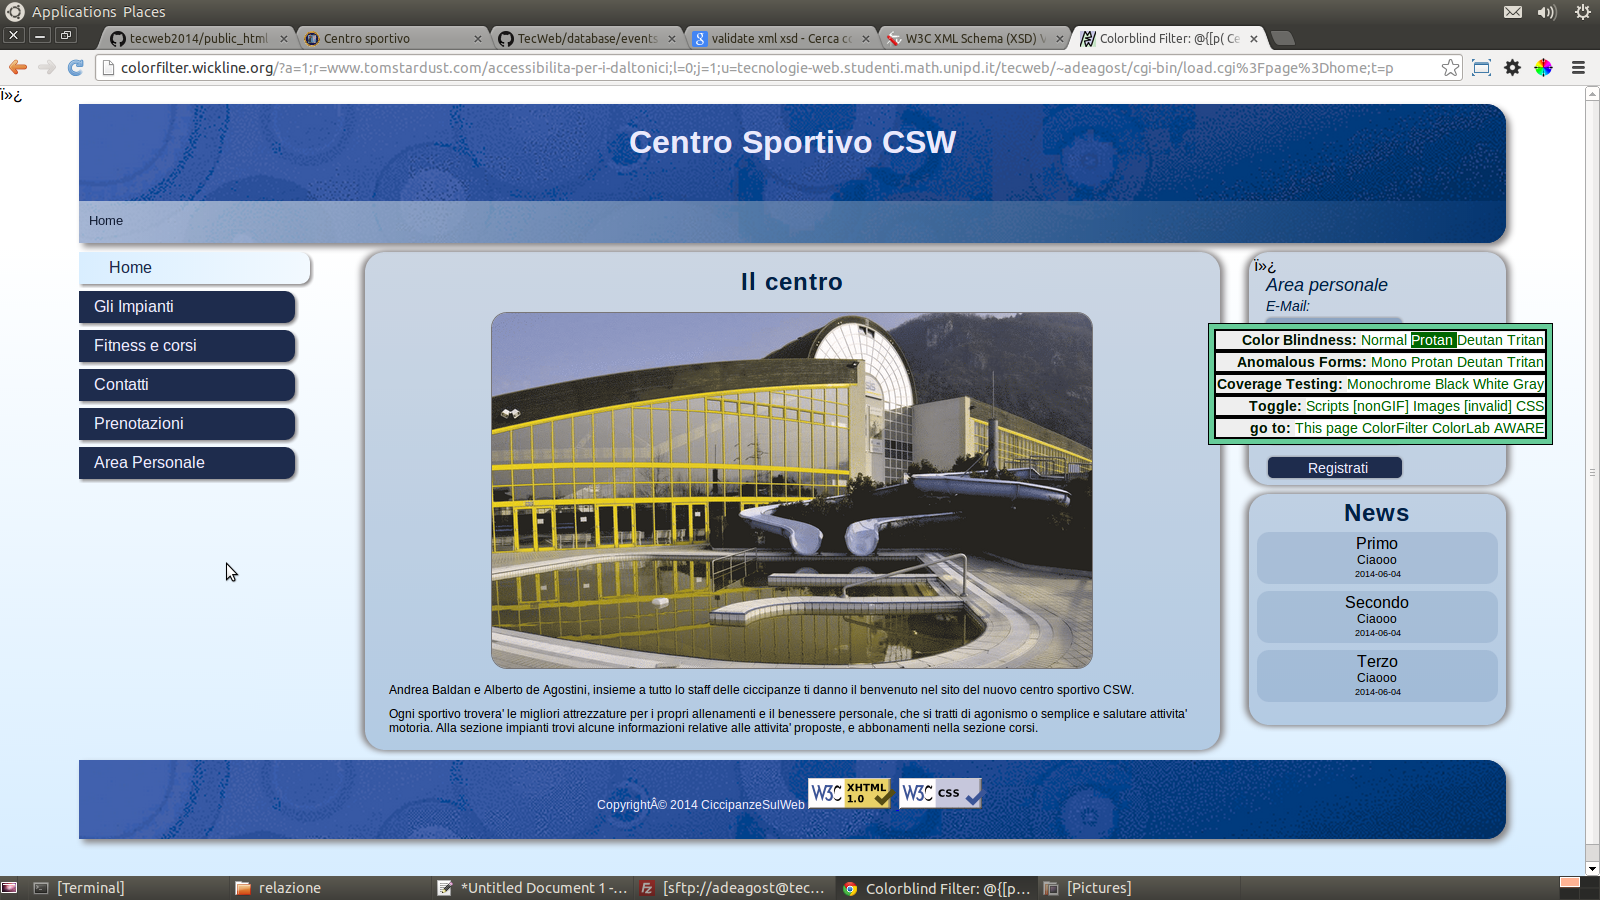
\includegraphics[width=0.8\textwidth]{images/protan.png} 
	\caption{a) protanopia}
\end{figure}
\begin{figure}[H]
	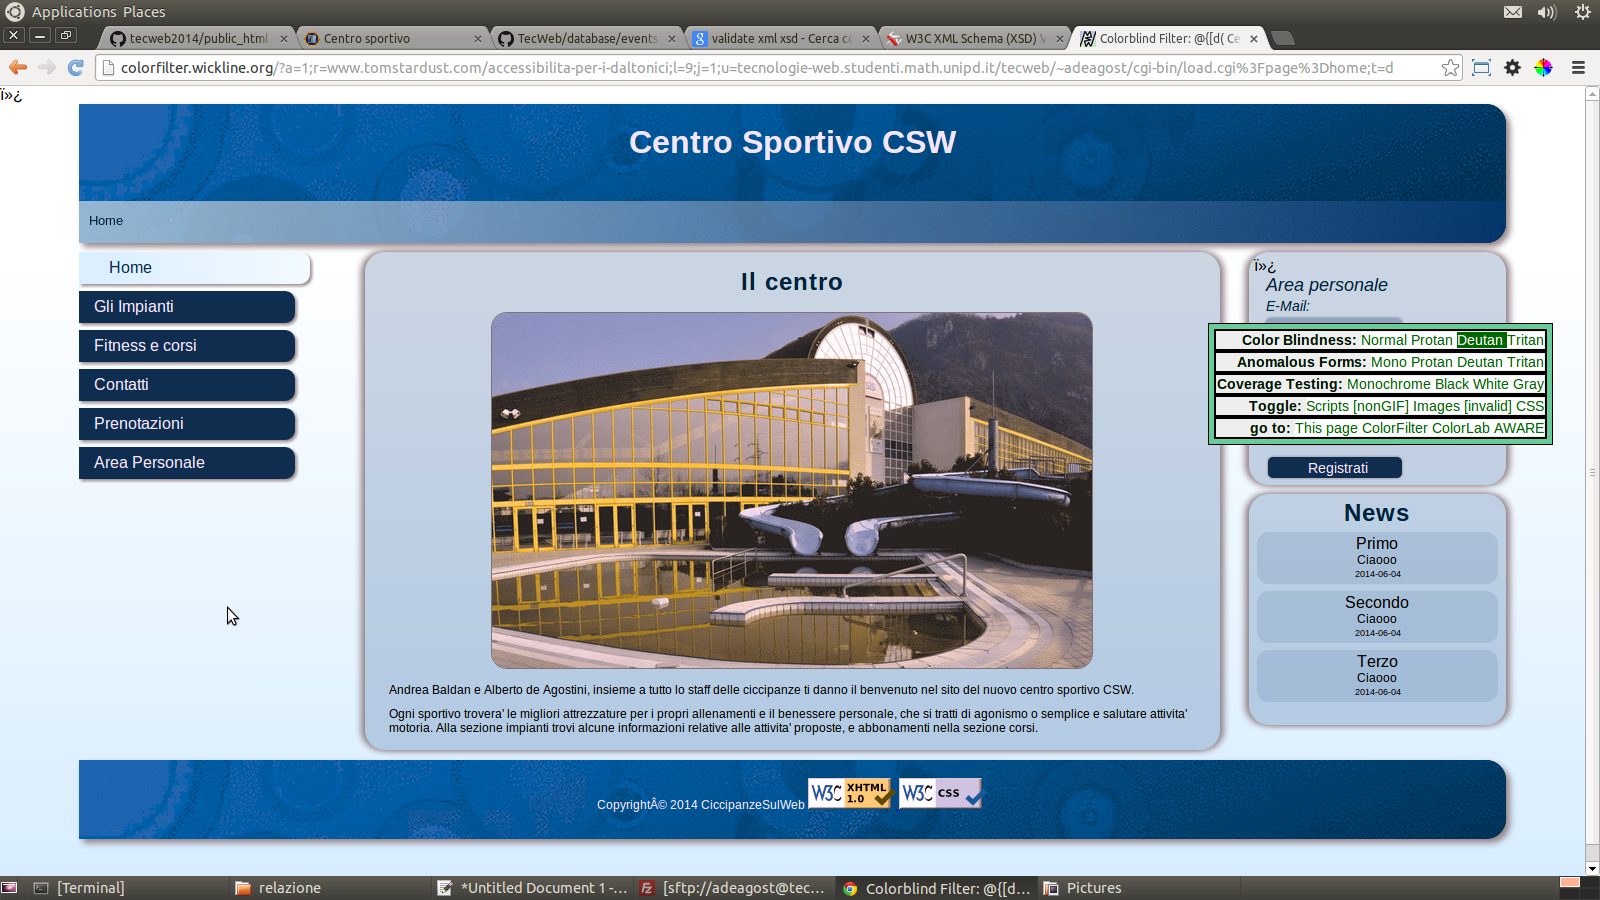
\includegraphics[width=0.8\textwidth]{images/deutran.png} 
	\caption{b) deutranopia} 
\end{figure}
\begin{figure}[H]
	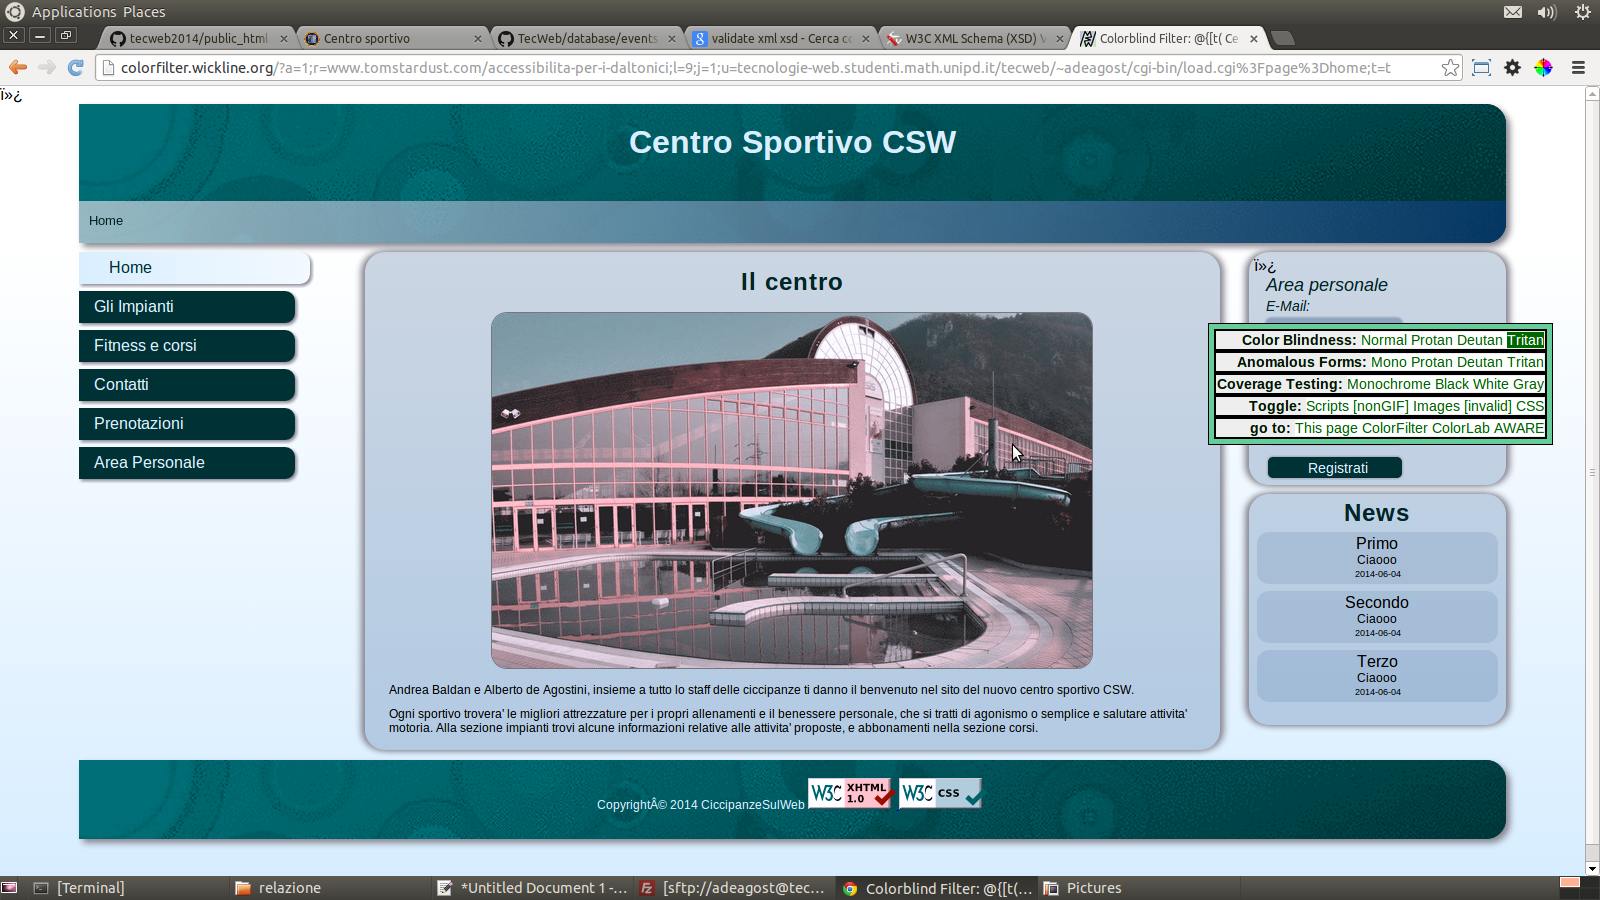
\includegraphics[width=0.8\textwidth]{images/tritan.png} 
	\caption{c) tritanopia}
\end{figure}
abbiamo allegato solo poche immagini visto che i colori utilizzati nel sito sono sempre gli stessi in ogni pagina.\newline
Abbiamo controllato anche il contrasto del sito su \newline \textbf{http://gmazzocato.altervista.org/colorwheel/wheel.php} per scegliere colori con contrasto ratio sempre maggiore di 7 per avere un punteggio di AAA. Su quel sito si puo' vedere anche il contrasto sempre per le persone che soffrono di protanopia, deutranopia e tritanopia.

\subsection{Accessibilita' tramite tastiera}
Un sito per essere accessibile deve essere completamente navigabile anche solo tramite tastiera, la navigazione tramite tastiera nel nostro sito risulta essere lineare e non difficile. Abbiamo inserito prima del \textbf{\#Nav} un link nascosto per saltare direttamente al contenuto per chi non voglia scorrere tutto il menu' di navigazione, lo stesso abbiamo fatto all'inizio del contenuto ove troviamo un altro link nascosto per saltare direttamente al menu' di login cosi' da poter arrivare al menu' login per effettuare l'accesso con soli 2 "salti" per gli utenti che gia' avendo un account vogliono direttamente effettuare un operazione.
Per questi due link nascosti abbiamo utilizzato \texttt{Tabindex} in modo da prioriticizzarli rispetto al resto del sito per favorire una navigazione piu' rapida agli utenti piu' esperti. 
\subsection{Accessibilita' per ciechi}
Abbiamo effettuato test con 4 diversi screen reader:
\begin{itemize}
	\item Jaws
	\item NVDA
	\item Chromevox
	\item Fangs for Firefox
\end{itemize}
La navigazione tramite screen reader risulta essere lineare e non presentare evidenti problemi tuttavia abbiamo notato che ogni screen reader utilizza regole diverse e con qualcuno risulta essere piu' di facile comprensione.
Con NVDA e Jaws abbiamo riscontrato una lettura del sito migliore e una piu' facile navigabilita', con ChromeVox la navigazione ci e' risultata essere piu' difficile tuttavia non e' un vero e proprio screen reader e abbiamo trovato in internet diverse valutazioni negative a riguardo.
Per quanto riguarda Fangs non e' un vero screen reader ma un emulatore di screen reader, ovvero renderizza la pagina come sarebbe letta dallo screen reader dando quindi in output una pagina solamente testuale lineare con le informazioni che sarebbero lette.
Una differenza sostanziale la troviamo quando lo screen reader va a leggere la tablella degli orari dei corsi:\newline
\begin{figure}[H]
	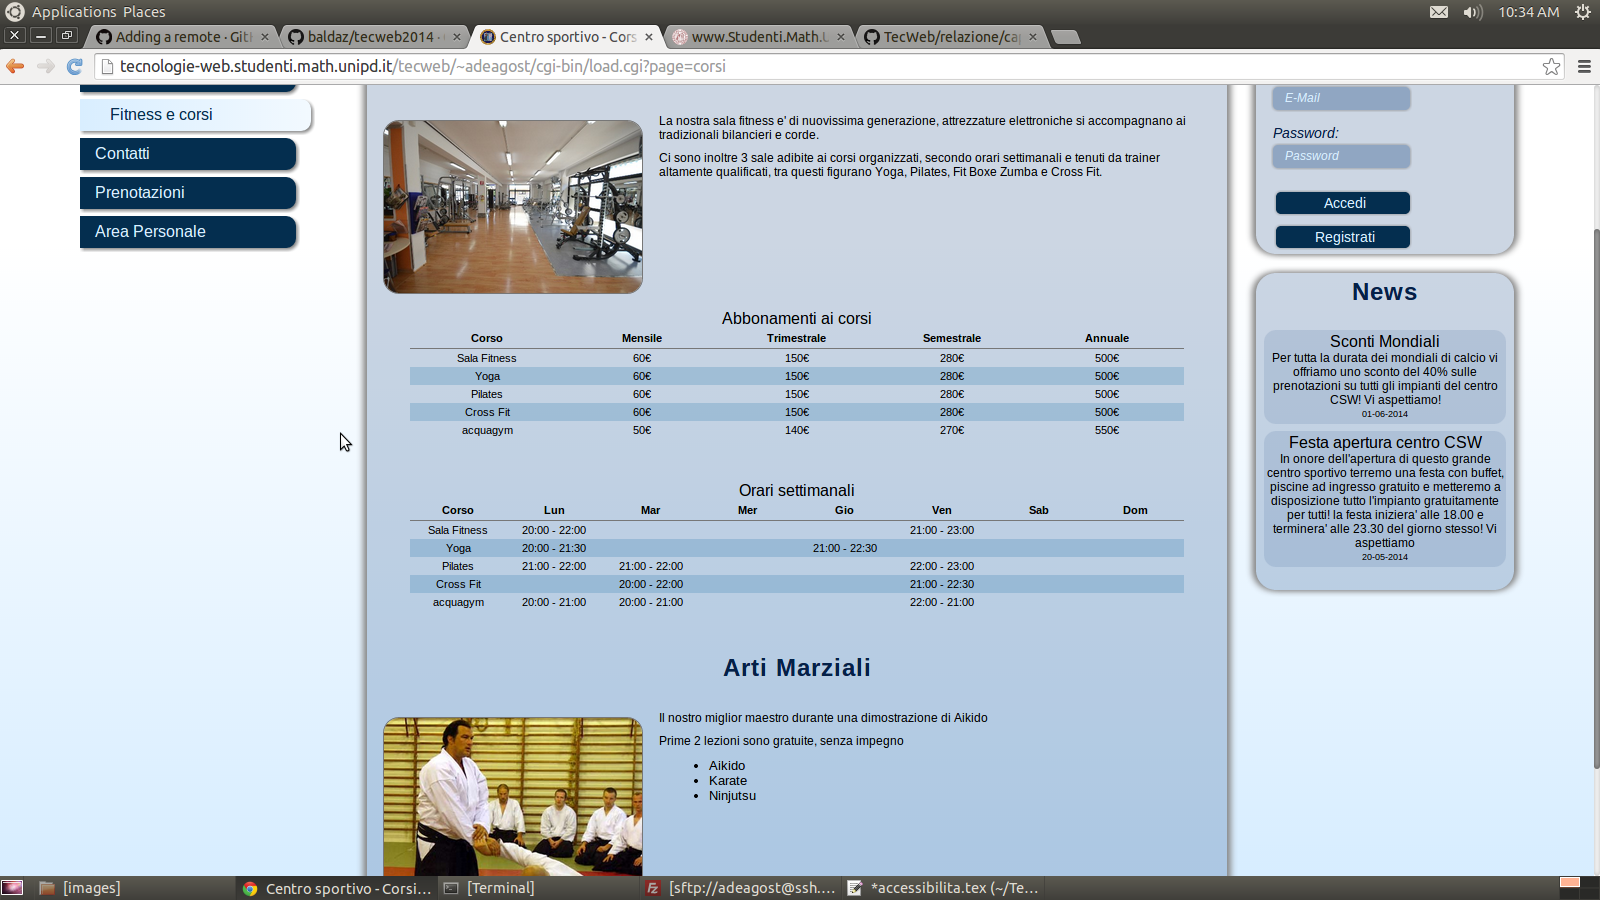
\includegraphics[height=0.4\textwidth]{images/tabella_corsi.png} 
\end{figure}
poiche' con Jaws e NVDA la lettura risulta essere 'giusta' mentre con ChromeVox le caselle vuote vengono saltate compromettendo la comprensione della tabella.
\paragraph{Total Validator}
Abbiamo usato Total Validator per la validazione del nostro sito visto le sue regole stringenti e conformi agli standard WCAG 2.0 AAA. Due errori sono stati riscontrati e non corretti per le motivazioni sottostanti:
\begin{itemize}
	\item Attributo \<time\> non supportato
	\item Attributo \<placeholder\> non supportato
\end{itemize}
Entrambi i tag appena riportati sono stati introdotti in \texttt{HTML5} e percio' non conformi, tuttavia abbiamo deciso di non eliminarli dal sito poiche' entrambi hanno un azione di fallback elegante poiche' quando un browser non supporta \texttt{placeholder} semplicemente o non c'e' testo (placeholder text) nella \texttt{textbox} o il testo e' semplicemente nero.
L'attributo \texttt{time} lo abbiamo lasciato poiche' visualmente non risulta visibile all'utente tuttavia screenreader quali Jaws e NVDA leggono le informazioni interne a \<time\> \</time\> nel modo giusto. 
Esempio "ore \<time\>18:00\</time\>" viene letto 'ore diciotto e zero zero' mentre "ore 18:00" viene letto 'ore diciotto duepunti zero zero' o su alcuni screen reader 'ore milleottocento'.
Per questi motivi abbiamo deciso di lasciare questi tag all'interno nel nostro sito.

\subsection{Accessibilita' parte amministrativa}
La parte amministrativa del nostro sito risulta essere molto semplice e intuitiva.
Abbiamo tralasciato volutamente la parte 'estetica' amministrativa per creare pagine piu' facili da capire.\newline
Tuttavia non abbiamo provato la parte amministrativa con screenreader per mancanza di tempo.
\subsection{Lingua}
Essendo il sito di un centro sportivo locale abbiamo deciso di localizzarlo solamente in lingua italiana.

\section{CSS}

Per lo sviluppo di un sito web il ramo della presentazione risulta molto importante. Abbiamo cercato di creare un layout fluido, semplice ed intuitivo per tutti considerando che ogni persona e' un potenziale cliente come gia' mezionato nel capitolo di analizi utenza.
Il sito e' diviso fondamentalmente in 6 sezioni:
\begin{itemize}
	\item \textbf{Header} sempre nella parte superiore della pagina contiene il Titolo del centro sportivo e \textbf{Path} che risulta utile quando si accede alla pagina per la registrazione e durante la prenotazione di un campo poiche' sono 2 pagine di 'secondo livello'
	\item	\textbf{Navigation} consiste nel menu' con tutti i link utili per la navigazione nel sito
	\item \textbf{Content} sempre al centro della pagina consiste nel contenuto del sito, contiene tutte le informazioni utili, la pagina di registrazione e tutti i form per la prenotazione dei campi da gioco.
	\item \textbf{Login} presente in ogni pagina contiene un piccolo form per effettuare l'accesso al sito o un link per andare alla registrazione per un nuovo utente.
	\item \textbf{News} e' un piccolo riquadro con le varie news inserite dall'amministratore
	\item \textbf{footer} posto sempre nella parte inferiore del sito contiene le immagini delle varie validazioni.
\end{itemize}

\subsection{Differenze su diversi terminali}

Abbiamo utilizzato le \textbf{mediaquery} per ottenere diversi layouts su vari terminali.
qui sotto riportiamo delle immagini per mostrare alcune di queste differenze:

\begin{figure}
	{\centering 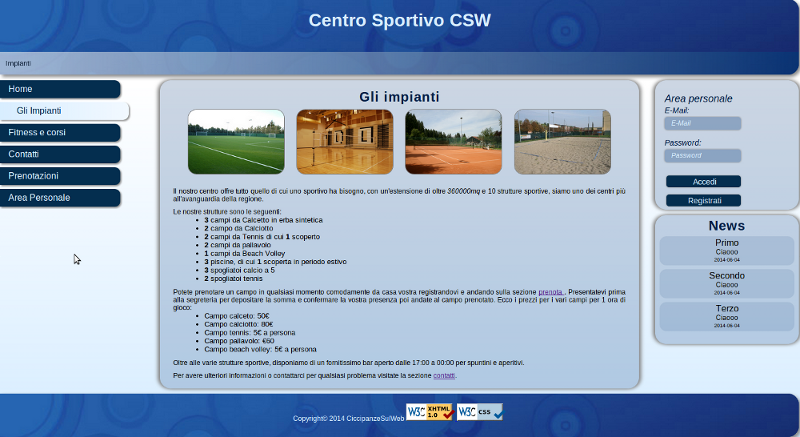
\includegraphics[height=0.3\textwidth]{images/normal.png} 
	\caption{a) style}}
\end{figure}
\begin{figure}
	{\centering 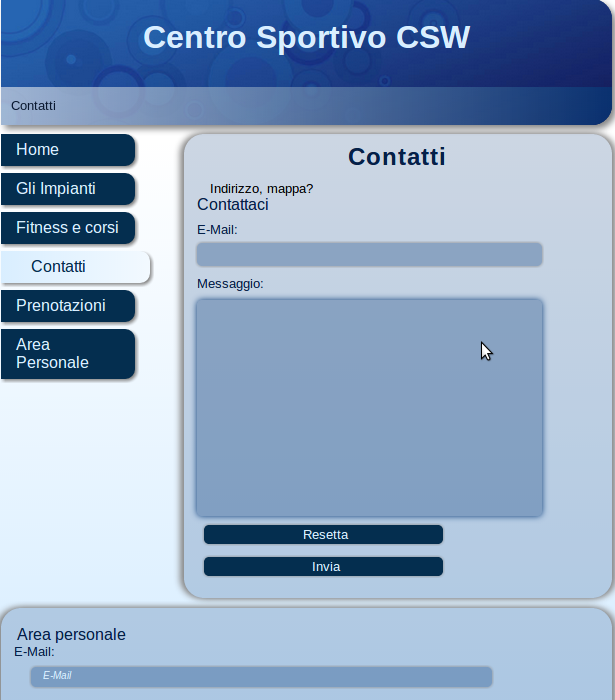
\includegraphics[height=0.3\textwidth]{images/tablet.png} 
	\caption{b) tablet} }
\end{figure}
\begin{figure}
	{\centering 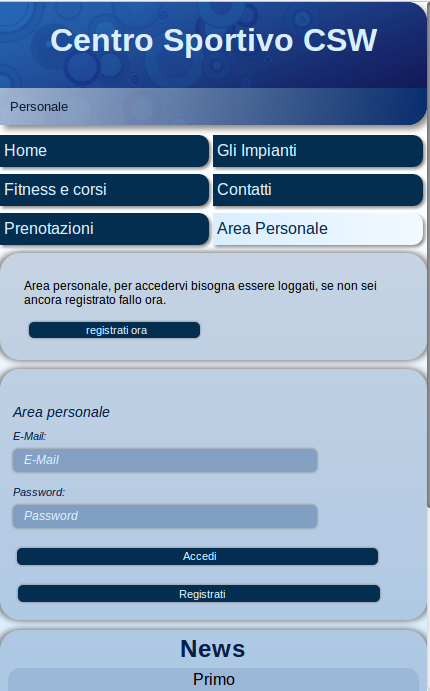
\includegraphics[height=0.3\textwidth]{images/mobile.png} 
	\caption{c) mobile}}
\end{figure}

Su dispositivi con risoluzioni alte abbiamo deciso di usare un layout a 3 colonne mentre come possiamo notare su dispositivi con media risoluzione come tablet abbiamo deciso di spostare semplicemente la parte Login e News sotto per lasciare piu' spazio al contenuto essendo di maggiore importanza.
Su dispositivi mobile abbiamo messo tutto in colonna.

\subsection{Compatibilita'}

Nello sviluppo della parte di presentazioni abbiamo usato qualche regola CSS non compatibile con tutti i browsers o non con tutte le versioni.
Per un maggior supporto abbiamo utilizzato diversi \textbf{vendor prefix} quali \textbf{-moz},\textbf{-o},\textbf{-webkit}
Per la compatibilita' di queste regole abbiamo effettuato delle ricerche online e basandoci su alcuni siti come \textbf{http://caniuse.com/}.
possiamo ad esempio vedere la compatibilita' di 'Transition' nei vari browser cosi': \newline \newline
 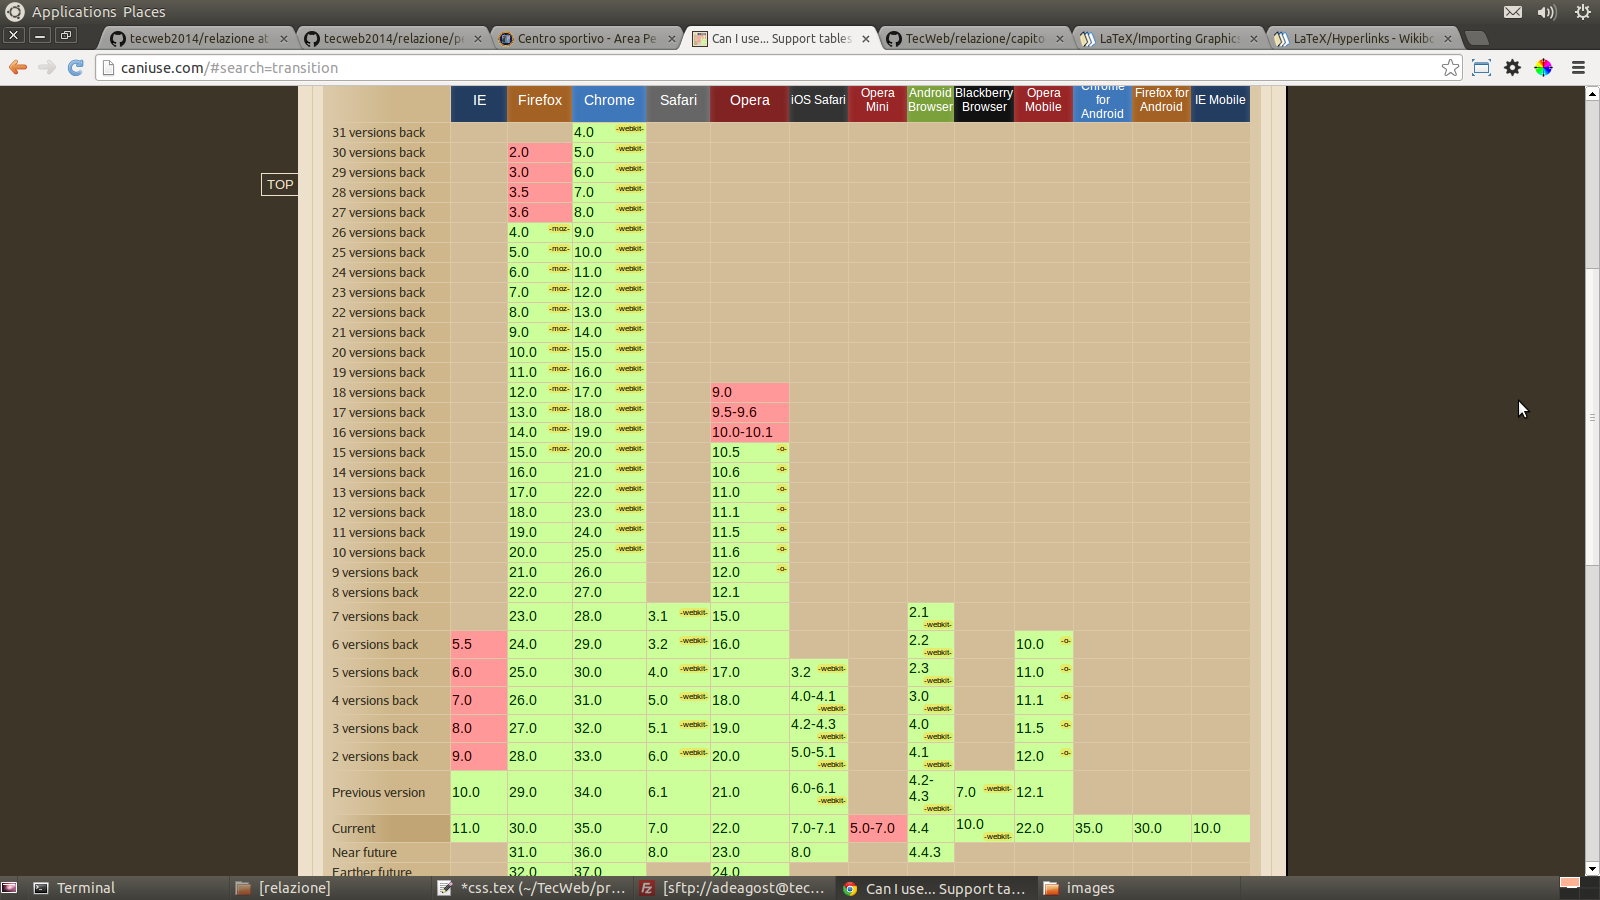
\includegraphics[width=0.7\textwidth]{images/caniuse1.png} \newline
Altre regole sono:
\begin{itemize}
	\item rgba che ha un 90\% di compatibilita' globale
	\item border-radius usato per arrotondare header, footer e varie immagini e' supportato da tutti i browser eccetto opera mini, da IE9 e da firefox con prefisso -moz fino alla versione 3.6 anche senza successivamente.
	\item box-shadow supportato da tutte le versione recenti di tutti i browser eccetto opera mini, mentre per alcune versioni vecchie servono prefissi come -webkit per chrome fino a versione 9
\end{itemize}

In ogni caso anche con versioni che non supportano queste regole css abbiamo visto che c'e' sempre un fallback elegante, il sito risulta essere meno accattivante tuttavia il funzionamento e la dispozione generale del sito non cambiano rimanendo cosi' accettabile con ogni browser.\newline
Per i test di compatibilita' sono stati effettuati con tutti i browser che sono presenti nel laboratorio Paolotti che sono i seguenti:
\begin{itemize}
	\item chrome versione 34.0 nessun problema
	\item chromium versione 34.0 nessun problema
	\item firefox versione 28.0 nessun problema
	\item konqueror versione 4.5 con questo browser la navigazione e' pressoche' impossibile, si riscontrano molti problemi quali il non supporto a nessuna delle regole css precedentemente elencate, non rispetta il ridimensionamento delle immagini, alcuni link addirittura risultano non funzionanti.
Tuttavia dopo alcune ricerche in internet abbiamo deciso deliberatamente di tralasciarlo viste le bassissime percentuali di utilizzo nel mondo.
	\item Opera versione 12.16 salvo qualche differenza come il colore dei placeholder tutto risulta funzionare normalmente.
	\item Internet Explorer
	\item Safari
\end{itemize}

Abbiamo anche effettuato test con Chrome disabilitando tutti gli stili o eliminando tutte le immagini e la navigazione sul sito non risultava compromessa.

\section{Perl}

\subsection{Organizzazione}

Trattandosi di un sito con una buona quantità di contenuti dinamici, è stato studiato un approccio quanto più modularizzato possibile, in modo da garantire maggior chiarezza e manutenibilità, una sorta di \textit{pattern MVC}, dove le \textit{view} sono rappresentate da templates (\texttt{.tmpl}) raccolti in una directory completamente separata dal codice, modelli e controller sono contenuti in 3 file contenenti inoltre le funzioni principali necessarie al popolamento dinamico del sito, si è quindi resa necessaria la suddivisione di esse in una gerarchia formata da tre moduli:

\begin{itemize}

  \item \texttt{UTILS} classe padre principale, raccoglie le funzioni di uso generale per il funzionamento e la popolazione delle varie pagine, caricamento ed interfaccia dei vari database XML (Model)
  \item \texttt{UTILS::Admin} classe figlio di UTILS, raccoglie le funzioni strettamente necessarie al backend dell'applicazione, funzionalità di login e mantenimento delle sessioni
  \item \texttt{UTILS::UserService} classe figlio di UTILS, raccoglie le funzioni necessarie al compimento delle operazioni strettamente legate all'utente (e.g CRUD delle proprie generalità), prenotazione risorse

\end{itemize} \newline
Alcune funzioni all'interno di questi moduli sono state ``privatizzate'', in quanto funzioni di utilità non direttamente finalizzate all'utilizzo da parte dell'utente (e.g. creazione scheletro tabelle, calcolo e conversione dei giorni della settimana etc.). 
In particolare ognuno di questi moduli fa da appoggio a rispettivi script utilizzati per effettuare le varie operazione per mezzo di dispatch tables, che consentono di risparmiare un gran numero di operazioni ridondanti e di automatizzare il piu possibile le operazioni da eseguire, aumentando inoltre la separazione tra codice e contenuto, avvicinandosi ad un approccio MVC:

\begin{itemize}

  \item \texttt{load.cgi} si appoggia ad \texttt{UTILS} ed è il motore di popolamento principale del sito, ogni pagina accessibile è generata e popolata da questo script, per mezzo di dispatch tables
  \item \texttt{admin.cgi} si appoggia ad \texttt{UTILS::Admin}, controparte backend di \texttt{load.cgi}, ogni pagina della parte amministrativa è generata da questo script
  \item \texttt{process.pl} script necessario alle basilari operazioni di modifica/popolamento risorse/pagine (CRUD)
  \item \texttt{user\_jobs.pl} controparte frontend di \texttt{process.pl}, tutte le operazioni che l'utente può effettuare sono gestite da questo codice

\end{itemize}
\newline
Vi sono infine \texttt{login.pl}, \texttt{login.cgi} e \texttt{logout.pl}, piccoli script atti solo all'autenticazione dell'utente, \textit{frontend} e \textit{backend} ed alla chiusura di eventuali sessioni aperte.
\texttt{vbooked.pl} è infine lo script utilizzato per visualizzare le tabelle di prenotazione via AJAX senza il bisogno di effettuare \textit{refresh} della pagina.


\subsection{Sistema di popolamento templates}

Ogni \textit{route} richiama il \textit{dispatcher} da \texttt{UTILS} e passa un \textit{hash} contenente i parametri necessari al popolamento del template richiamato, che inoltre possiede lo stesso nome della \textit{route} appunto.\newline
Da \texttt{load.cgi} attraverso l'oggetto \texttt{\$utils} e la dispatch table viene automaticamente richiamato e popolato il template corretto: \newline \newline
\small{\textit{Dispatch table} all'interno di \texttt{load.cgi}:}


\scriptsize{
\begin{verbatim}

    my %routes = (
      'home'          => \&index,
      'impianti'      => \&impianti,
      'contatti'      => \&contatti,
      'corsi'         => \&corsi,
      'prenotazioni'  => \&prenotazioni,
      'registrazione' => \&registrazione,
      'personale'     => \&personale,
      'prenota'       => \&prenota,
      'edit_personal' => \&edit_personal
    );

    if( grep { $page eq $_} keys %routes){
      $routes{$page}->();
    }

\end{verbatim}
}

\small{Funzione \texttt{corsi} associata alla route corsi:}

\scriptsize{
\begin{verbatim}
   sub corsi {
     my @loop_prices = $utils->list_prices;
     my @loop_scheduling = $utils->list_scheduling;
     my %params = (
	title => 'Centro sportivo - Corsi',
	page      => 'corsi',
	path      => 'Corsi',
	courses_price => \@loop_prices,
	courses_scheduling => \@loop_scheduling,
	LOGIN     => $sess_params{is_logged},
	USER      => $sess_params{profile},
	attempt   => $sess_params{attempt}
	);
     $utils->dispatcher('corsi', %params);
   }
\end{verbatim}
}\newline
\small{Funzione \texttt{dispatcher} all'interno di \texttt{UTILS.pm}, avendo per convenzione \texttt{\$route} il nome del template a cui la route è associata, esso viene richiamato e popolato con i parametri contenuti in \texttt{\%params} settati nella funzione \texttt{corsi} in \texttt{load.cgi}:}
 
\scriptsize{
\begin{verbatim}
   sub dispatcher {
     my $self = shift;
     my $route = shift;
     my %params = @_;
     my $template = HTML::Template->new(filename => $route.".tmpl", utf8 => 1);
     foreach(keys %params){
        $template->param($_ => $params{$_});
     }	
     my @loop_news = $self->getNews;
     foreach(@loop_news){
        delete $_->{N_ID};
     }
     $template->param(NEWS => @loop_news);
     print "Content-Type: text/html\n\n", $template->output;
   }
\end{verbatim}
}

\section{Note e difficolta' riscontrate}
\subsection{Difficolta'}
Il problema piu' grosso che abbiamo avuto e' stato il fatto di dover completare il progetto in due membri anziche' tre.
Alcune feature come ad esempio una traduzione in inglese sono state tralasciate per via del elevato carico di lavoro.\newline
Un iniziale scelta dello schema di colori nel layout ha creato problemi nella parte di accessibilita' e siamo stati costretti a cambiarlo.

\subsection{Note}
La parte amministrativa e' rudimentale e un po' scarna sempre per la mancanza di tempo, abbiamo pensato di fare solo una validazione tramite Javascript in questa sezione poiche' si presume che l'amministratore del sito sia informato a dovere e abbia un idea giusta del contenuto che andra' a mettere nel proprio sito (ad esempio nei corsi evitare di sovrascrivere gli orari in qualche giorno e' sua responsabilita').\newline
Abbiamo deciso di separare la parte amministrativa dal sito per scelte di sicurezza (\textit{information hiding}).
Nel nostro sito l'utilizzo di \texttt{javascript} e' limitato alla validazione dei dati nei vari form e al sistema di visualizzazione delle tabelle di prenotazione senza bisogno di refresh (\texttt{AJAX}).\newline
Sono stati effettuati i test nel caso venga disabilitato \texttt{javascript} nel sito, come fallback ci sono controlli lato server via \texttt{Perl} e un button per il refresh della pagina per la visualizzazione delle tabelle di prenotazione sempre via \texttt{Perl}.\newline 

%etc
\end{document}
